\PassOptionsToPackage{unicode=true}{hyperref} % options for packages loaded elsewhere
\PassOptionsToPackage{hyphens}{url}
%
\documentclass[]{book}
\usepackage{lmodern}
\usepackage{amssymb,amsmath}
\usepackage{ifxetex,ifluatex}
\usepackage{fixltx2e} % provides \textsubscript
\ifnum 0\ifxetex 1\fi\ifluatex 1\fi=0 % if pdftex
  \usepackage[T1]{fontenc}
  \usepackage[utf8]{inputenc}
  \usepackage{textcomp} % provides euro and other symbols
\else % if luatex or xelatex
  \usepackage{unicode-math}
  \defaultfontfeatures{Ligatures=TeX,Scale=MatchLowercase}
\fi
% use upquote if available, for straight quotes in verbatim environments
\IfFileExists{upquote.sty}{\usepackage{upquote}}{}
% use microtype if available
\IfFileExists{microtype.sty}{%
\usepackage[]{microtype}
\UseMicrotypeSet[protrusion]{basicmath} % disable protrusion for tt fonts
}{}
\IfFileExists{parskip.sty}{%
\usepackage{parskip}
}{% else
\setlength{\parindent}{0pt}
\setlength{\parskip}{6pt plus 2pt minus 1pt}
}
\usepackage{hyperref}
\hypersetup{
            pdftitle={Codes for STEM},
            pdfauthor={Noushin Nabavi},
            pdfborder={0 0 0},
            breaklinks=true}
\urlstyle{same}  % don't use monospace font for urls
\usepackage{color}
\usepackage{fancyvrb}
\newcommand{\VerbBar}{|}
\newcommand{\VERB}{\Verb[commandchars=\\\{\}]}
\DefineVerbatimEnvironment{Highlighting}{Verbatim}{commandchars=\\\{\}}
% Add ',fontsize=\small' for more characters per line
\usepackage{framed}
\definecolor{shadecolor}{RGB}{248,248,248}
\newenvironment{Shaded}{\begin{snugshade}}{\end{snugshade}}
\newcommand{\AlertTok}[1]{\textcolor[rgb]{0.94,0.16,0.16}{#1}}
\newcommand{\AnnotationTok}[1]{\textcolor[rgb]{0.56,0.35,0.01}{\textbf{\textit{#1}}}}
\newcommand{\AttributeTok}[1]{\textcolor[rgb]{0.77,0.63,0.00}{#1}}
\newcommand{\BaseNTok}[1]{\textcolor[rgb]{0.00,0.00,0.81}{#1}}
\newcommand{\BuiltInTok}[1]{#1}
\newcommand{\CharTok}[1]{\textcolor[rgb]{0.31,0.60,0.02}{#1}}
\newcommand{\CommentTok}[1]{\textcolor[rgb]{0.56,0.35,0.01}{\textit{#1}}}
\newcommand{\CommentVarTok}[1]{\textcolor[rgb]{0.56,0.35,0.01}{\textbf{\textit{#1}}}}
\newcommand{\ConstantTok}[1]{\textcolor[rgb]{0.00,0.00,0.00}{#1}}
\newcommand{\ControlFlowTok}[1]{\textcolor[rgb]{0.13,0.29,0.53}{\textbf{#1}}}
\newcommand{\DataTypeTok}[1]{\textcolor[rgb]{0.13,0.29,0.53}{#1}}
\newcommand{\DecValTok}[1]{\textcolor[rgb]{0.00,0.00,0.81}{#1}}
\newcommand{\DocumentationTok}[1]{\textcolor[rgb]{0.56,0.35,0.01}{\textbf{\textit{#1}}}}
\newcommand{\ErrorTok}[1]{\textcolor[rgb]{0.64,0.00,0.00}{\textbf{#1}}}
\newcommand{\ExtensionTok}[1]{#1}
\newcommand{\FloatTok}[1]{\textcolor[rgb]{0.00,0.00,0.81}{#1}}
\newcommand{\FunctionTok}[1]{\textcolor[rgb]{0.00,0.00,0.00}{#1}}
\newcommand{\ImportTok}[1]{#1}
\newcommand{\InformationTok}[1]{\textcolor[rgb]{0.56,0.35,0.01}{\textbf{\textit{#1}}}}
\newcommand{\KeywordTok}[1]{\textcolor[rgb]{0.13,0.29,0.53}{\textbf{#1}}}
\newcommand{\NormalTok}[1]{#1}
\newcommand{\OperatorTok}[1]{\textcolor[rgb]{0.81,0.36,0.00}{\textbf{#1}}}
\newcommand{\OtherTok}[1]{\textcolor[rgb]{0.56,0.35,0.01}{#1}}
\newcommand{\PreprocessorTok}[1]{\textcolor[rgb]{0.56,0.35,0.01}{\textit{#1}}}
\newcommand{\RegionMarkerTok}[1]{#1}
\newcommand{\SpecialCharTok}[1]{\textcolor[rgb]{0.00,0.00,0.00}{#1}}
\newcommand{\SpecialStringTok}[1]{\textcolor[rgb]{0.31,0.60,0.02}{#1}}
\newcommand{\StringTok}[1]{\textcolor[rgb]{0.31,0.60,0.02}{#1}}
\newcommand{\VariableTok}[1]{\textcolor[rgb]{0.00,0.00,0.00}{#1}}
\newcommand{\VerbatimStringTok}[1]{\textcolor[rgb]{0.31,0.60,0.02}{#1}}
\newcommand{\WarningTok}[1]{\textcolor[rgb]{0.56,0.35,0.01}{\textbf{\textit{#1}}}}
\usepackage{longtable,booktabs}
% Fix footnotes in tables (requires footnote package)
\IfFileExists{footnote.sty}{\usepackage{footnote}\makesavenoteenv{longtable}}{}
\usepackage{graphicx,grffile}
\makeatletter
\def\maxwidth{\ifdim\Gin@nat@width>\linewidth\linewidth\else\Gin@nat@width\fi}
\def\maxheight{\ifdim\Gin@nat@height>\textheight\textheight\else\Gin@nat@height\fi}
\makeatother
% Scale images if necessary, so that they will not overflow the page
% margins by default, and it is still possible to overwrite the defaults
% using explicit options in \includegraphics[width, height, ...]{}
\setkeys{Gin}{width=\maxwidth,height=\maxheight,keepaspectratio}
\setlength{\emergencystretch}{3em}  % prevent overfull lines
\providecommand{\tightlist}{%
  \setlength{\itemsep}{0pt}\setlength{\parskip}{0pt}}
\setcounter{secnumdepth}{5}
% Redefines (sub)paragraphs to behave more like sections
\ifx\paragraph\undefined\else
\let\oldparagraph\paragraph
\renewcommand{\paragraph}[1]{\oldparagraph{#1}\mbox{}}
\fi
\ifx\subparagraph\undefined\else
\let\oldsubparagraph\subparagraph
\renewcommand{\subparagraph}[1]{\oldsubparagraph{#1}\mbox{}}
\fi

% set default figure placement to htbp
\makeatletter
\def\fps@figure{htbp}
\makeatother

\usepackage{booktabs}
\usepackage[]{natbib}
\bibliographystyle{plainnat}

\title{Codes for STEM}
\author{Noushin Nabavi}
\date{2020-09-10}

\begin{document}
\maketitle

{
\setcounter{tocdepth}{1}
\tableofcontents
}
\hypertarget{coding-for-stem}{%
\chapter{Coding for STEM}\label{coding-for-stem}}

\begin{quote}
Tools and capabilities of data science is changing everyday!
\end{quote}

This is how I understand it today:

\textbf{Data can:}
* Describe the current state of an organization or process\\
* Detec anomalous events\\
* Diagnose the causes of events and behaviors\\
* Predict future events

\textbf{Data Science workflows can be developed for: }\\
* Data collection and management\\
* Exploration and visualization\\
* Experimentation and prediction

\textbf{Applications of data science can include: }\\
* Traditional machine learning: e.g.~finding probabilities of events, labeled data, and algorithms\\
* Deep learning: neurons work together for image and natural language recognition but requires more training data\\
* Internet of things (IOT): e.g.~smart watch algorithms to detect and analyze motion sensors

\textbf{Data science teams can consist of:}
* Data engineers: SQL, Java, Scala, Python\\
* Data analysts: Dashboards, hypothesis tests and visualization using spreadsheets, SQL, BI (Tableau, power BI, looker)\\
* Machine learning scientists: predictions and extrapolations, classification, etc. and use R or python * Data employees can be isolated, embedded, or hybrid

Data use can come with risks of identification of personal information. Policies for personally identifiable information may need to consider:\\
* sensitivity and caution\\
* pseudonymization and anonymization

Preferences can be stated or revealed through the data so questions need to be specific, avoid loaded language, calibrate, require actionable results.

\textbf{Data storage and retrieval may include: }
* parallel storage solutions (e.g.~cluster or server)\\
* cloud storage (google, amazon, azure)\\
* types of data: 1) unstructured (email, text, video, audio, web, and social media = document database); 2) structured = relational databases\\
* Data querying: NoSQL and SQL

\textbf{Communication of data can include: }\\
* Dashboards\\
* Markdowns\\
* BI tools\\
* rshiny or d3.js

\textbf{Team management around data can use: }
* Trello, slack, rocket chat, or JIRA to communicate due data and priority

\textbf{A/B Testing: }
* Control and Variation in samples\\
* 4 steps in A/B testing: pick metric to track, calculate sample size, run the experiment, and check significance

Machine learning (ML) can be used for time series forecasting (investigate seasonality on any time scale), natural language processing (word count, word embeddings to create features that group similar words), neural networks, deep learning, and AI.\\
\textbf{Learning can be classified into: }
\emph{Supervised}: labels and features/ Model evaluation on test and train data with applications in:
* recommendation systems\\
* subscription predictions\\
* email subject optimization\\
\emph{Unsupervised}: unlabeled data with only features\\
* clustering

\textbf{Deep learning and AI requirements: }
* prediction is more feasible than explanations\\
* lots of very large amount of training data

\hypertarget{introduction}{%
\chapter{Introduction}\label{introduction}}

\hypertarget{r-for-reporting}{%
\chapter{R for Reporting}\label{r-for-reporting}}

Possible ways to report your findings include e-mailing figures and tables around with some explanatory text or creating reports in Word, LaTeX or HTML.

R code used to produce the figures and tables is typically not part of these documents. So in case the data changes, e.g., if new data becomes available, the code needs to be re-run and all the figures and tables updated. This can be rather cumbersome. If code and reporting are not in the same place, it can also be a bit of a hassle to reconstruct the details of the analysis carried out to produce the results.

To enable reproducible data analysis and research, the idea of dynamic reporting is that data, code and results are all in one place. This can for example be a R Markdown document like this one. Generating the report automatically executes the analysis code and includes the results in the report.

\hypertarget{usage-demonstrations}{%
\section{Usage demonstrations}\label{usage-demonstrations}}

\hypertarget{inline-code}{%
\subsection{Inline code}\label{inline-code}}

Simple pieces of code can be included inline. This can be handy to, e.g., include the number of observations in your data set dynamically. The \emph{cars} data set, often used to illustrate the linear model, has 50 observations.

\hypertarget{code-chunks}{%
\subsection{Code chunks}\label{code-chunks}}

You can include typical output like a summary of your data set and a summary of a linear model through code chunks.

\begin{Shaded}
\begin{Highlighting}[]
\KeywordTok{summary}\NormalTok{(cars)}
\end{Highlighting}
\end{Shaded}

\begin{verbatim}
##      speed           dist       
##  Min.   : 4.0   Min.   :  2.00  
##  1st Qu.:12.0   1st Qu.: 26.00  
##  Median :15.0   Median : 36.00  
##  Mean   :15.4   Mean   : 42.98  
##  3rd Qu.:19.0   3rd Qu.: 56.00  
##  Max.   :25.0   Max.   :120.00
\end{verbatim}

\begin{Shaded}
\begin{Highlighting}[]
\NormalTok{m <-}\StringTok{ }\KeywordTok{lm}\NormalTok{(dist }\OperatorTok{~}\StringTok{ }\NormalTok{speed, }\DataTypeTok{data =}\NormalTok{ cars)}
\KeywordTok{summary}\NormalTok{(m)}
\end{Highlighting}
\end{Shaded}

\begin{verbatim}
## 
## Call:
## lm(formula = dist ~ speed, data = cars)
## 
## Residuals:
##     Min      1Q  Median      3Q     Max 
## -29.069  -9.525  -2.272   9.215  43.201 
## 
## Coefficients:
##             Estimate Std. Error t value Pr(>|t|)    
## (Intercept) -17.5791     6.7584  -2.601   0.0123 *  
## speed         3.9324     0.4155   9.464 1.49e-12 ***
## ---
## Signif. codes:  0 '***' 0.001 '**' 0.01 '*' 0.05 '.' 0.1 ' ' 1
## 
## Residual standard error: 15.38 on 48 degrees of freedom
## Multiple R-squared:  0.6511,	Adjusted R-squared:  0.6438 
## F-statistic: 89.57 on 1 and 48 DF,  p-value: 1.49e-12
\end{verbatim}

\hypertarget{include-tables}{%
\subsubsection{Include tables}\label{include-tables}}

The estimated coefficients, as well as their standard errors, t-values and p-values can also be included in the form of a table, for example through \textbf{knitr}'s \texttt{kable} function.

\begin{Shaded}
\begin{Highlighting}[]
\KeywordTok{library}\NormalTok{(}\StringTok{"knitr"}\NormalTok{)}
\KeywordTok{kable}\NormalTok{(}\KeywordTok{summary}\NormalTok{(m)}\OperatorTok{$}\NormalTok{coef, }\DataTypeTok{digits =} \DecValTok{2}\NormalTok{)}
\end{Highlighting}
\end{Shaded}

\begin{tabular}{l|r|r|r|r}
\hline
  & Estimate & Std. Error & t value & Pr(>|t|)\\
\hline
(Intercept) & -17.58 & 6.76 & -2.60 & 0.01\\
\hline
speed & 3.93 & 0.42 & 9.46 & 0.00\\
\hline
\end{tabular}

\hypertarget{include-figures}{%
\subsubsection{Include figures}\label{include-figures}}

The \textbf{trackeR} package provides infrastructure for running and cycling data in \textbf{R} and is used here to illustrate how figures can be included.

\begin{Shaded}
\begin{Highlighting}[]
\CommentTok{## install.packages("devtools")}
\CommentTok{## devtools::install_github("hfrick/trackeR")}
\KeywordTok{library}\NormalTok{(}\StringTok{"trackeR"}\NormalTok{) }
\KeywordTok{data}\NormalTok{(}\StringTok{"runs"}\NormalTok{, }\DataTypeTok{package =} \StringTok{"trackeR"}\NormalTok{)}
\end{Highlighting}
\end{Shaded}

A plot of how heart rate and pace evolve over time in 10 training sessions looks like this

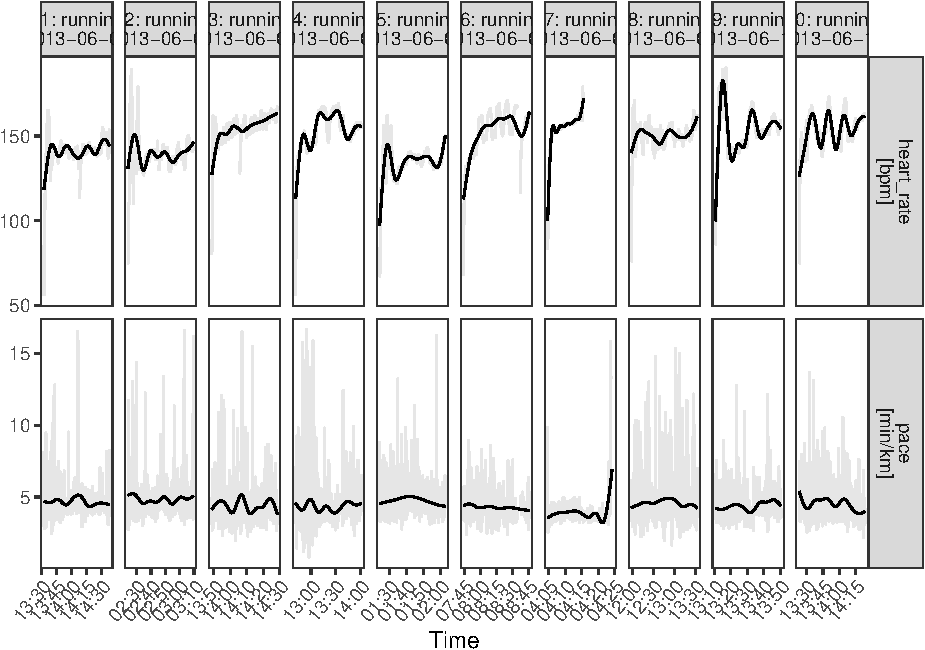
\includegraphics{code4stem_files/figure-latex/unnamed-chunk-4-1.pdf}

but the plot looks better with a wider plotting window.

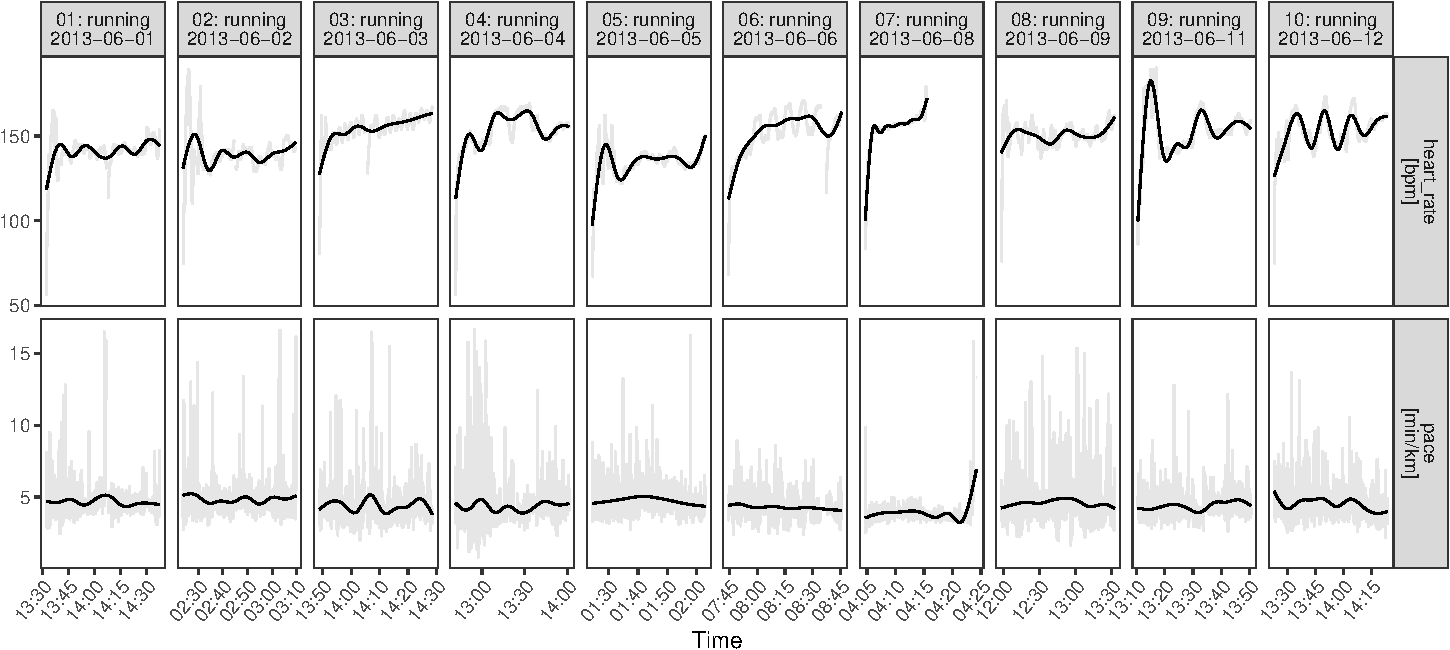
\includegraphics{code4stem_files/figure-latex/unnamed-chunk-5-1.pdf}

\hypertarget{resources}{%
\section{Resources}\label{resources}}

\begin{itemize}
\tightlist
\item
  \href{http://daringfireball.net/projects/markdown/}{Markdown main page}
\item
  \href{http://rmarkdown.rstudio.com/}{R Markdown}
\item
  \href{http://kbroman.org/knitr_knutshell/}{knitr in a nutshell} tutorial by Karl Broman
\end{itemize}

\hypertarget{useful-r-functions-examples}{%
\chapter{Useful R Functions + Examples}\label{useful-r-functions-examples}}

\begin{quote}
This is \emph{NOT} intended to be fully comprehensive list of every useful R function that exists, but is a practical demonstration of selected relevant examples presented in user-friendly format, all available in base R. For a wider collection to work through, this Reference Card is recommended: \url{https://cran.r-project.org/doc/contrib/Baggott-refcard-v2.pdf}
\end{quote}

\begin{quote}
Additional CRAN reference cards and R guides (including non-English documentation) found here: \url{https://cran.r-project.org/other-docs.html}
\end{quote}

\hypertarget{contents}{%
\section{Contents}\label{contents}}

A. Essentials\\
* 1. \texttt{getwd()}, \texttt{setwd()}\\
* 2. \texttt{?foo}, \texttt{help(foo)}, \texttt{example(foo)}\\
* 3. \texttt{install.packages("foo")}, \texttt{library("foo")}\\
* 4. \texttt{devtools::install\_github("username/packagename")}\\
* 5. \texttt{data("foo")}\\
* 6. \texttt{read.csv}, \texttt{read.table}\\
* 7. \texttt{write.table()}\\
* 8. \texttt{save()}, \texttt{load()}

B. Basics\\
* 9. \texttt{c()}, \texttt{cbind()}, \texttt{rbind()}, \texttt{matrix()}\\
* 10. \texttt{length()}, \texttt{dim()}\\
* 11. \texttt{sort()}, \texttt{\textquotesingle{}vector\textquotesingle{}{[}{]}}, \texttt{\textquotesingle{}matrix\textquotesingle{}{[}{]}}\\
* 12. \texttt{data.frame()}, \texttt{class()}, \texttt{names()}, \texttt{str()}, \texttt{summary()}, \texttt{View()}, \texttt{head()}, \texttt{tail()}, \texttt{as.data.frame()}

C. Core\\
* 13. \texttt{df{[}order(),{]}}\\
* 14. \texttt{df{[},c(){]}}, \texttt{df{[}which(),{]}}\\
* 15. \texttt{table()}\\
* 16. \texttt{mean()}, \texttt{median()}, \texttt{sd()}, \texttt{var()}, \texttt{sum()}, \texttt{min()}, \texttt{max()}, \texttt{range()}\\
* 17. \texttt{apply()}\\
* 18. \texttt{lapply()} using \texttt{list()}\\
* 19. \texttt{tapply()}

D. Common\\
* 20. \texttt{if} statement, \texttt{if...else} statement\\
* 21. \texttt{for} loop\\
* 22. \texttt{function()...}

\hypertarget{r-syntax}{%
\section{R Syntax}\label{r-syntax}}

\emph{REMEMBER: KEY R LANGUAGE SYNTAX}

\begin{itemize}
\tightlist
\item
  \textbf{Case Sensitivity}: as per most UNIX-based packages, R is case sensitive, hence \texttt{X} and \texttt{x} are different symbols and would refer to different variables.\\
\item
  \textbf{Expressions vs Assignments}: an expression, like \texttt{3\ +\ 5} can be given as a command which will be evaluated and the value immediately printed, but not stored. An assignment however, like \texttt{sum\ \textless{}-\ 3\ +\ 5} using the assignment operator \texttt{\textless{}-} also evaluates the expression \texttt{3\ +\ 5}, but instead of printing and not storing, it stores the value in the object \texttt{sum} but doesn't print the result. The object \texttt{sum} would need to be called to print the result.\\
\item
  \textbf{Reserved Words}: choice for naming objects is almost entirely free, except for these reserved words: \url{https://stat.ethz.ch/R-manual/R-devel/library/base/html/Reserved.html}\\
\item
  \textbf{Spacing}: outside of the function structure, spaces don't matter, e.g. \texttt{3+5} is the same as \texttt{3+\ \ \ \ \ 5} is the same as \texttt{3\ +\ 5}. For more best-practices for R code Hadley Wickham's Style Guide is a useful reference: \url{http://adv-r.had.co.nz/Style.html}
\item
  \textbf{Comments}: add comments within your code using a hastag, \texttt{\#}. R will ignore everything to the right of the hashtag within that line
\end{itemize}

\hypertarget{functional-examples}{%
\section{Functional examples}\label{functional-examples}}

\begin{enumerate}
\def\labelenumi{\arabic{enumi}.}
\tightlist
\item
  Working Directory management
\end{enumerate}

\begin{itemize}
\tightlist
\item
  \texttt{getwd()}, \texttt{setwd()}
  R/RStudio is always pointed at a specific directory on your computer, so it's important to be able to check what's the current directory using \texttt{getwd()}, and to be able to change and specify a different directory to work in using \texttt{setwd()}.
\end{itemize}

\#check the directory R is currently pointed at
getwd()

\begin{enumerate}
\def\labelenumi{\arabic{enumi}.}
\setcounter{enumi}{1}
\tightlist
\item
  Bring up help documentation \& examples
\end{enumerate}

\begin{itemize}
\tightlist
\item
  \texttt{?foo}, \texttt{help(foo)}, \texttt{example(foo)}
\end{itemize}

\begin{Shaded}
\begin{Highlighting}[]
\NormalTok{?boxplot}
\KeywordTok{help}\NormalTok{(boxplot)}
\KeywordTok{example}\NormalTok{(boxplot)}
\end{Highlighting}
\end{Shaded}

\begin{center}\rule{0.5\linewidth}{0.5pt}\end{center}

\begin{enumerate}
\def\labelenumi{\arabic{enumi}.}
\setcounter{enumi}{2}
\tightlist
\item
  Load \& Call CRAN Packages
\end{enumerate}

\begin{itemize}
\tightlist
\item
  \texttt{install.packages("foo")}, \texttt{library("foo")}
  Packages are add-on functionality built for R but not pre-installed (base R), hence you need to install/load the packages you want yourself. The majority of packages you'd want have been submitted to and are available via CRAN. At time of writing, the CRAN package repository featured 8,592 available packages.
\end{itemize}

\begin{enumerate}
\def\labelenumi{\arabic{enumi}.}
\setcounter{enumi}{3}
\tightlist
\item
  Load \& Call Packages from GitHub
\end{enumerate}

\begin{itemize}
\tightlist
\item
  \texttt{devtools::install\_github("username/packagename")}
  Not all packages you'll want will be available via CRAN, and you'll likely need to get certain packages from GitHub accounts. This example shows how to install the \texttt{shinyapps} package from RStudio's GitHub account.
\item
  install.packages(``devtools'') \#pre-requisite for \texttt{devtools...} function
\item
  devtools::install\_github(``rstudio/shinyapps'') \#install specific package from specific GitHub account
\item
  library(``shinyapps'') \#Call package
\end{itemize}

\begin{enumerate}
\def\labelenumi{\arabic{enumi}.}
\setcounter{enumi}{4}
\tightlist
\item
  Load datasets from base R \& Loaded Packages
\end{enumerate}

\begin{itemize}
\tightlist
\item
  \texttt{data("foo")}
\end{itemize}

\begin{Shaded}
\begin{Highlighting}[]
\CommentTok{#AIM: show available datasets}
\KeywordTok{data}\NormalTok{() }

\CommentTok{#AIM: load an available dataset}
\KeywordTok{data}\NormalTok{(}\StringTok{"iris"}\NormalTok{) }
\end{Highlighting}
\end{Shaded}

\begin{center}\rule{0.5\linewidth}{0.5pt}\end{center}

\begin{enumerate}
\def\labelenumi{\arabic{enumi}.}
\setcounter{enumi}{5}
\tightlist
\item
  I/O Loading Existing Local Data
\end{enumerate}

\begin{itemize}
\tightlist
\item
  \texttt{read.csv}, \texttt{read.table}
\end{itemize}

\begin{enumerate}
\def\labelenumi{(\alph{enumi})}
\tightlist
\item
  I/O When already in the working directory where the data is
\end{enumerate}

Import a local \textbf{csv} file (i.e.~where data is separated by \textbf{commas}), saving it as an object:
- object \textless{}- read.csv(``xxx.csv'')

Import a local tab delimited file (i.e.~where data is separated by \textbf{tabs}), saving it as an object:
- object \textless{}- read.csv(``xxx.csv'', header = FALSE)
---

\begin{enumerate}
\def\labelenumi{(\alph{enumi})}
\setcounter{enumi}{1}
\tightlist
\item
  I/O When NOT in the working directory where the data is
\end{enumerate}

For example to import and save a local \textbf{csv} file from a different working directory you either need to specify the file path (operating system specific), e.g.:

on a mac:
- object \textless{}- read.csv(``\textasciitilde{}/Desktop/R/data.csv'')

on windows:
= object \textless{}- read.csv(``C:/Desktop/R/data.csv'')

OR

You can use the file.choose() command which will interactively open up the file dialog box for you to browse and select the local file, e.g.:
- object \textless{}- read.csv(file.choose())

\begin{enumerate}
\def\labelenumi{(\alph{enumi})}
\setcounter{enumi}{2}
\tightlist
\item
  I/O Copying \& Pasting Data
\end{enumerate}

For relatively small amounts of data you can do an equivalent copy paste (operating system specific):

on a mac:
- object \textless{}- read.table(pipe(``pbpaste''))

on windows:
- object \textless{}- read.table(file = ``clipboard'')

\begin{enumerate}
\def\labelenumi{(\alph{enumi})}
\setcounter{enumi}{3}
\tightlist
\item
  I/O Loading Non-Numerical Data - character strings
\end{enumerate}

Be careful when loading text data! R may assume character strings are statistical factor variables, e.g. ``low'', ``medium'', ``high'', when are just individual labels like names. To specify text data NOT to be converted into factor variables, add \texttt{stringsAsFactor\ =\ FALSE} to your \texttt{read.csv/read.table} command:
- object \textless{}- read.table(``xxx.txt'', stringsAsFactors = FALSE)

\begin{enumerate}
\def\labelenumi{(\alph{enumi})}
\setcounter{enumi}{4}
\tightlist
\item
  I/O Downloading Remote Data
\end{enumerate}

For accessing files from the web you can use the same \texttt{read.csv/read.table} commands. However, the file being downloaded does need to be in an R-friendly format (maximum of 1 header row, subsequent rows are the equivalent of one data record per row, no extraneous footnotes etc.). Here is an example downloading an online csv file of coffee harvest data used in a Nature study:
- object \textless{}- read.csv(``\url{http://sumsar.net/files/posts/2014-02-04-bayesian-first-aid-one-sample-t-test/roubik_2002_coffe_yield.csv}'')

\begin{enumerate}
\def\labelenumi{\arabic{enumi}.}
\setcounter{enumi}{6}
\tightlist
\item
  I/O Exporting Data Frame
\end{enumerate}

\begin{itemize}
\tightlist
\item
  \texttt{write.table()}
\end{itemize}

Navigate to the working directory you want to save the data table into, then run the command (in this case creating a tab delimited file):
- write.table(object, ``xxx.txt'', sep = "\t")

\begin{enumerate}
\def\labelenumi{\arabic{enumi}.}
\setcounter{enumi}{7}
\tightlist
\item
  I/O Saving Down \& Loading Objects
\end{enumerate}

\begin{itemize}
\tightlist
\item
  \texttt{save()}, \texttt{load()}
\end{itemize}

These two commands allow you to save a named R object to a file and restore that object again.\\
Navigate to the working directory you want to save the object in then run the command:
- save(object, file = ``xxx.rda'')

reload the object:
- load(``xxx.rda'')

\begin{enumerate}
\def\labelenumi{\arabic{enumi}.}
\setcounter{enumi}{8}
\tightlist
\item
  Vector \& Matrix Construction
\end{enumerate}

\begin{itemize}
\tightlist
\item
  \texttt{c()}, \texttt{cbind()}, \texttt{rbind()}, \texttt{matrix()}
  Vectors (lists) \& Matrices (two-dimensional arrays) are very common R data structures.
\end{itemize}

\begin{Shaded}
\begin{Highlighting}[]
\CommentTok{#use c() to construct a vector by concatenating data}
\NormalTok{foo <-}\StringTok{ }\KeywordTok{c}\NormalTok{(}\DecValTok{1}\NormalTok{, }\DecValTok{2}\NormalTok{, }\DecValTok{3}\NormalTok{, }\DecValTok{4}\NormalTok{) }\CommentTok{#example of a numeric vector}
\NormalTok{oof <-}\StringTok{ }\KeywordTok{c}\NormalTok{(}\StringTok{"A"}\NormalTok{, }\StringTok{"B"}\NormalTok{, }\StringTok{"C"}\NormalTok{, }\StringTok{"D"}\NormalTok{) }\CommentTok{#example of a character vector}
\NormalTok{ofo <-}\StringTok{ }\KeywordTok{c}\NormalTok{(}\OtherTok{TRUE}\NormalTok{, }\OtherTok{FALSE}\NormalTok{, }\OtherTok{TRUE}\NormalTok{, }\OtherTok{TRUE}\NormalTok{) }\CommentTok{#example of a logical vector}

\CommentTok{#use cbind() & rbind() to construct matrices}
\NormalTok{coof <-}\StringTok{ }\KeywordTok{cbind}\NormalTok{(foo, oof) }\CommentTok{#bind vectors in column concatenation to make a matrix}
\NormalTok{roof <-}\StringTok{ }\KeywordTok{rbind}\NormalTok{(foo, oof) }\CommentTok{#bind vectors in row concatenation to make a matrix}

\CommentTok{#use matrix() to construct matrices}
\NormalTok{moof <-}\StringTok{ }\KeywordTok{matrix}\NormalTok{(}\DataTypeTok{data =} \DecValTok{1}\OperatorTok{:}\DecValTok{12}\NormalTok{, }\DataTypeTok{nrow=}\DecValTok{3}\NormalTok{, }\DataTypeTok{ncol=}\DecValTok{4}\NormalTok{) }\CommentTok{#creates matrix by specifying set of values, no. of rows & no. of columns}
\end{Highlighting}
\end{Shaded}

\begin{enumerate}
\def\labelenumi{\arabic{enumi}.}
\setcounter{enumi}{9}
\tightlist
\item
  Vector \& Matrix Explore
\end{enumerate}

\begin{itemize}
\tightlist
\item
  \texttt{length()}, \texttt{dim()}
\end{itemize}

\begin{Shaded}
\begin{Highlighting}[]
\KeywordTok{length}\NormalTok{(foo) }\CommentTok{#length of vector}

\KeywordTok{dim}\NormalTok{(coof) }\CommentTok{#returns dimensions (no. of rows & columns) of vector/matrix/dataframe}
\end{Highlighting}
\end{Shaded}

\begin{enumerate}
\def\labelenumi{\arabic{enumi}.}
\setcounter{enumi}{10}
\tightlist
\item
  Vector \& Matrix Sort \& Select
\end{enumerate}

\begin{itemize}
\tightlist
\item
  \texttt{sort()}, \texttt{\textquotesingle{}vector\textquotesingle{}{[}{]}}, \texttt{\textquotesingle{}matrix\textquotesingle{}{[}{]}}
\end{itemize}

\begin{Shaded}
\begin{Highlighting}[]
\CommentTok{#create another numeric vector}
\NormalTok{jumble <-}\StringTok{ }\KeywordTok{c}\NormalTok{(}\DecValTok{4}\NormalTok{, }\DecValTok{1}\NormalTok{, }\DecValTok{2}\NormalTok{, }\DecValTok{3}\NormalTok{)}
\KeywordTok{sort}\NormalTok{(jumble) }\CommentTok{#sorts a numeric vector in ascending order (default)}
\KeywordTok{sort}\NormalTok{(jumble, }\DataTypeTok{decreasing =} \OtherTok{TRUE}\NormalTok{) }\CommentTok{#specify the decreasing arg to reverse default order}

\CommentTok{#create another character vector}
\NormalTok{mumble <-}\StringTok{ }\KeywordTok{c}\NormalTok{( }\StringTok{"D"}\NormalTok{, }\StringTok{"B"}\NormalTok{, }\StringTok{"C"}\NormalTok{, }\StringTok{"A"}\NormalTok{)}
\KeywordTok{sort}\NormalTok{(mumble) }\CommentTok{#sorts a character vector in alphabetical order (default)}
\KeywordTok{sort}\NormalTok{(mumble, }\DataTypeTok{decreasing =} \OtherTok{TRUE}\NormalTok{) }\CommentTok{#specify the decreasing arg to reverse default order}

\NormalTok{jumble[}\DecValTok{1}\NormalTok{] }\CommentTok{#selects first value in our jumble vector}
\KeywordTok{tail}\NormalTok{(jumble, }\DataTypeTok{n=}\DecValTok{1}\NormalTok{) }\CommentTok{#selects last value}
\NormalTok{jumble[}\KeywordTok{c}\NormalTok{(}\DecValTok{1}\NormalTok{,}\DecValTok{3}\NormalTok{)] }\CommentTok{#selects the 1st & 3rd values}
\NormalTok{jumble[}\OperatorTok{-}\KeywordTok{c}\NormalTok{(}\DecValTok{1}\NormalTok{,}\DecValTok{3}\NormalTok{)] }\CommentTok{#selects everything except the 1st & 3rd values}

\NormalTok{coof[}\DecValTok{1}\NormalTok{,] }\CommentTok{#selects the 1st row of our coof matrix}
\NormalTok{coof[,}\DecValTok{1}\NormalTok{] }\CommentTok{#selects the 1st column}
\NormalTok{coof[}\DecValTok{2}\NormalTok{,}\DecValTok{1}\NormalTok{] }\CommentTok{#selects the value in the 2nd row, 1st column}
\NormalTok{coof[,}\StringTok{"oof"}\NormalTok{] }\CommentTok{#selects the column named "oof"}
\NormalTok{coof[}\DecValTok{1}\OperatorTok{:}\DecValTok{3}\NormalTok{,] }\CommentTok{#selects columns 1 to 3 inclusive}
\NormalTok{coof[}\KeywordTok{c}\NormalTok{(}\DecValTok{1}\NormalTok{,}\DecValTok{2}\NormalTok{,}\DecValTok{3}\NormalTok{),] }\CommentTok{#selects the 1st, 2nd & 3rd rows (same as previous)}
\end{Highlighting}
\end{Shaded}

\begin{enumerate}
\def\labelenumi{\arabic{enumi}.}
\setcounter{enumi}{11}
\tightlist
\item
  Create \& Explore Data Frames
\end{enumerate}

\begin{itemize}
\tightlist
\item
  \texttt{data.frame()}, \texttt{class()}, \texttt{names()}, \texttt{str()}, \texttt{summary()}, \texttt{View()}, \texttt{head()}, \texttt{tail()}, \texttt{as.data.frame()}
  A data frame is a matrix-like data structure made up of lists of variables with the same number of rows, which can be of differing data types (numeric, character, factor etc.) - matrices must have columns all of the same data type.
\end{itemize}

\begin{Shaded}
\begin{Highlighting}[]
\CommentTok{#create a data frame with 3 columns with 4 rows each}
\NormalTok{doof <-}\StringTok{ }\KeywordTok{data.frame}\NormalTok{(}\StringTok{"V1"}\NormalTok{=}\DecValTok{1}\OperatorTok{:}\DecValTok{4}\NormalTok{, }\StringTok{"V2"}\NormalTok{=}\KeywordTok{c}\NormalTok{(}\StringTok{"A"}\NormalTok{,}\StringTok{"B"}\NormalTok{,}\StringTok{"C"}\NormalTok{,}\StringTok{"D"}\NormalTok{), }\StringTok{"V3"}\NormalTok{=}\DecValTok{5}\OperatorTok{:}\DecValTok{8}\NormalTok{)}

\KeywordTok{class}\NormalTok{(doof) }\CommentTok{#check data frame object class}
\KeywordTok{names}\NormalTok{(doof) }\CommentTok{# returns column names}
\KeywordTok{str}\NormalTok{(doof) }\CommentTok{#see structure of data frame}
\KeywordTok{summary}\NormalTok{(doof) }\CommentTok{#returns basic summary stats}
\KeywordTok{View}\NormalTok{(doof) }\CommentTok{#invokes spreadsheet-style viewer}
\KeywordTok{head}\NormalTok{(doof, }\DataTypeTok{n=}\DecValTok{2}\NormalTok{) }\CommentTok{#shows first parts of object, here requesting the first 2 rows}
\KeywordTok{tail}\NormalTok{(doof, }\DataTypeTok{n=}\DecValTok{2}\NormalTok{) }\CommentTok{#shows last parts of object, here requesting the last 2 rows}

\NormalTok{convert <-}\StringTok{ }\KeywordTok{as.data.frame}\NormalTok{(coof) }\CommentTok{#convert a non-data frame object into a data frame}
\end{Highlighting}
\end{Shaded}

\begin{enumerate}
\def\labelenumi{\arabic{enumi}.}
\setcounter{enumi}{12}
\tightlist
\item
  Data Frame Sort
\end{enumerate}

\begin{itemize}
\tightlist
\item
  \texttt{df{[}order(),{]}}
\end{itemize}

\begin{Shaded}
\begin{Highlighting}[]
\CommentTok{#use 'painters' data frame}
\KeywordTok{library}\NormalTok{(}\StringTok{"MASS"}\NormalTok{) }\CommentTok{#call package with the required data}
\KeywordTok{data}\NormalTok{(}\StringTok{"painters"}\NormalTok{) }\CommentTok{#load required data}
\KeywordTok{View}\NormalTok{(painters) }\CommentTok{#scan dataset}

\CommentTok{#syntax for using a specific variable: df=data frame, '$', V1=variable name}
\NormalTok{df}\OperatorTok{$}\NormalTok{V1 }

\CommentTok{#AIM: print the 'School' variable column}
\NormalTok{painters}\OperatorTok{$}\NormalTok{School}

\CommentTok{#syntax for df[order(),]}
\NormalTok{df[}\KeywordTok{order}\NormalTok{(df}\OperatorTok{$}\NormalTok{V1, df}\OperatorTok{$}\NormalTok{V2...),] }\CommentTok{#function arguments: df=data frame, in square brackets specify within the order() the columns with which to sort the ROWS by, where default ordering is Ascending, the tailing comma specifies returning all the columns in the df. If only certain columns are wanted this can be specified after the comma.}

\CommentTok{#AIM: order the dataset rows based on the painters' Composition Score column, in Ascending order}
\NormalTok{painters[}\KeywordTok{order}\NormalTok{(painters}\OperatorTok{$}\NormalTok{Composition),] }\CommentTok{#Composition is the sorting variable}

\CommentTok{#AIM: order the dataset rows based on the painters' Composition Score column, in Descending order}
\NormalTok{painters[}\KeywordTok{order}\NormalTok{(}\OperatorTok{-}\NormalTok{painters}\OperatorTok{$}\NormalTok{Composition),] }\CommentTok{#append a minus sign in front of the variable you want to sort by in Descending order}

\CommentTok{#AIM: order the dataset rows based on the painters' Composition Score column, in Descending order but return just the first 3 columns}
\NormalTok{painters[}\KeywordTok{order}\NormalTok{(}\OperatorTok{-}\NormalTok{painters}\OperatorTok{$}\NormalTok{Composition), }\KeywordTok{c}\NormalTok{(}\DecValTok{1}\OperatorTok{:}\DecValTok{3}\NormalTok{)]}
\end{Highlighting}
\end{Shaded}

\begin{enumerate}
\def\labelenumi{\arabic{enumi}.}
\setcounter{enumi}{13}
\tightlist
\item
  Data Frame Select \& Deselect
\end{enumerate}

\begin{itemize}
\tightlist
\item
  \texttt{df{[},c(){]}}, \texttt{df{[}which(),{]}}
\end{itemize}

\begin{Shaded}
\begin{Highlighting}[]
\CommentTok{#use 'painters' data frame}

\CommentTok{#syntax for select & deselect based on column variables}
\NormalTok{df[, }\KeywordTok{c}\NormalTok{(}\StringTok{"V1"}\NormalTok{, }\StringTok{"V2"}\NormalTok{...)] }\CommentTok{#function arguments: df=data frame, in square brackets specify columns to select or deselect. The comma specifies returning all the rows. If certain rows are wanted this can be specified before the comma.}

\CommentTok{#AIM: select the Composition & Drawing variables based on their column name}
\NormalTok{painters[, }\KeywordTok{c}\NormalTok{(}\StringTok{"Composition"}\NormalTok{, }\StringTok{"Drawing"}\NormalTok{)] }\CommentTok{#subset the df, selecting just the named columns (and all the rows)}

\CommentTok{#AIM: select the Composition & Drawing variables based on their column positions in the painters data frame}
\NormalTok{painters[, }\KeywordTok{c}\NormalTok{(}\DecValTok{1}\NormalTok{,}\DecValTok{2}\NormalTok{)] }\CommentTok{#subset the df, selecting just the 1st & 2nd columns (and all the rows)}

\CommentTok{#AIM: drop the Expression variable based on it's column position in the painters data frame and return just the first 5 rows}
\NormalTok{painters[}\KeywordTok{c}\NormalTok{(}\DecValTok{1}\OperatorTok{:}\DecValTok{5}\NormalTok{), }\DecValTok{-4}\NormalTok{] }\CommentTok{#returns the subsetted df having deselected the 4th column, Expression and the first 5 rows}


\CommentTok{#syntax for select & deselect based on row variable values}
\NormalTok{df[}\KeywordTok{which}\NormalTok{(),] }\CommentTok{#df=data frame, specify the variable value within the `which()` to subset the df on. Again, the tailing comma specifies returning all the columns. If certain columns are wanted this can be specified after the comma.}

\CommentTok{#AIM: select all rows where the painters' School is the 'A' category}
\NormalTok{painters[}\KeywordTok{which}\NormalTok{(painters}\OperatorTok{$}\NormalTok{School }\OperatorTok{==}\StringTok{ "A"}\NormalTok{),] }\CommentTok{#returns the subsetted df where equality holds true, i.e. row value in School variable column is 'A'}

\CommentTok{#AIM: deselect all rows where the painters' School is the 'A' category, i.e. return df subset without 'A' values, AND also only select rows where Colour score > 10}
\NormalTok{painters[}\KeywordTok{which}\NormalTok{(painters}\OperatorTok{$}\NormalTok{School }\OperatorTok{!=}\StringTok{ "A"} \OperatorTok{&}\StringTok{ }\NormalTok{painters}\OperatorTok{$}\NormalTok{Colour }\OperatorTok{>}\StringTok{ }\DecValTok{10}\NormalTok{),] }\CommentTok{#returns the subsetted df where equality holds true, i.e. row value in School variable column is 'not A', AND the Colour score filter is also true.}
\end{Highlighting}
\end{Shaded}

\begin{enumerate}
\def\labelenumi{\arabic{enumi}.}
\setcounter{enumi}{14}
\tightlist
\item
  Data Frame Frequency Calculations
\end{enumerate}

\begin{itemize}
\tightlist
\item
  \texttt{table()}
\end{itemize}

\begin{Shaded}
\begin{Highlighting}[]
\CommentTok{#create new data frame}
\NormalTok{flavour <-}\StringTok{ }\KeywordTok{c}\NormalTok{(}\StringTok{"choc"}\NormalTok{, }\StringTok{"strawberry"}\NormalTok{, }\StringTok{"vanilla"}\NormalTok{, }\StringTok{"choc"}\NormalTok{, }\StringTok{"strawberry"}\NormalTok{, }\StringTok{"strawberry"}\NormalTok{) }
\NormalTok{gender <-}\StringTok{ }\KeywordTok{c}\NormalTok{(}\StringTok{"F"}\NormalTok{, }\StringTok{"F"}\NormalTok{, }\StringTok{"M"}\NormalTok{, }\StringTok{"M"}\NormalTok{, }\StringTok{"F"}\NormalTok{, }\StringTok{"M"}\NormalTok{)}
\NormalTok{icecream <-}\StringTok{ }\KeywordTok{data.frame}\NormalTok{(flavour, gender) }\CommentTok{#icecream df made up of 2 factor variables, flavour & gender, with 3 & 2 levels respectively (choc/strawberry/vanilla & F/M)}

\CommentTok{#AIM: create a frequency distribution table which shows the count of each gender in the df}
\KeywordTok{table}\NormalTok{(icecream}\OperatorTok{$}\NormalTok{gender) }

\CommentTok{#AIM: create a frequency distribution table which shows the count of each flavour in the df}
\KeywordTok{table}\NormalTok{(icecream}\OperatorTok{$}\NormalTok{flavour)}

\CommentTok{#AIM: create Contingency/2-Way Table showing the counts for each combination of flavour & gender level }
\KeywordTok{table}\NormalTok{(icecream}\OperatorTok{$}\NormalTok{flavour, icecream}\OperatorTok{$}\NormalTok{gender)}
\end{Highlighting}
\end{Shaded}

\begin{enumerate}
\def\labelenumi{\arabic{enumi}.}
\setcounter{enumi}{15}
\tightlist
\item
  Descriptive/Summary Stats Functions
\end{enumerate}

\begin{itemize}
\tightlist
\item
  \texttt{mean()}, \texttt{median()}, \texttt{sd()}, \texttt{var()}, \texttt{sum()}, \texttt{min()}, \texttt{max()}, \texttt{range()}
\end{itemize}

\begin{Shaded}
\begin{Highlighting}[]
\CommentTok{#re-using the jumble vector from before}
\NormalTok{jumble <-}\StringTok{ }\KeywordTok{c}\NormalTok{(}\DecValTok{4}\NormalTok{, }\DecValTok{1}\NormalTok{, }\DecValTok{2}\NormalTok{, }\DecValTok{3}\NormalTok{) }

\KeywordTok{mean}\NormalTok{(jumble)}
\KeywordTok{median}\NormalTok{(jumble)}
\KeywordTok{sd}\NormalTok{(jumble)}
\KeywordTok{var}\NormalTok{(jumble)}
\KeywordTok{sum}\NormalTok{(jumble)}
\KeywordTok{min}\NormalTok{(jumble)}
\KeywordTok{max}\NormalTok{(jumble)}
\KeywordTok{range}\NormalTok{(jumble)}
\end{Highlighting}
\end{Shaded}

\begin{enumerate}
\def\labelenumi{\arabic{enumi}.}
\setcounter{enumi}{16}
\tightlist
\item
  Apply Functions
\end{enumerate}

\begin{itemize}
\tightlist
\item
  \texttt{apply()}
  \texttt{apply()} returns a vector, array or list of values where a specified function has been applied to the `margins' (rows/cols combo) of the original vector/array/list.
\end{itemize}

\begin{Shaded}
\begin{Highlighting}[]
\CommentTok{#re-using the moof matrix from before}
\NormalTok{moof <-}\StringTok{ }\KeywordTok{matrix}\NormalTok{(}\DataTypeTok{data =} \DecValTok{1}\OperatorTok{:}\DecValTok{12}\NormalTok{, }\DataTypeTok{nrow=}\DecValTok{3}\NormalTok{, }\DataTypeTok{ncol=}\DecValTok{4}\NormalTok{) }

\CommentTok{#apply syntax}
\KeywordTok{apply}\NormalTok{(X, MARGIN, FUN,...) }\CommentTok{#function arguments: X=an array, MARGIN=1 to apply to rows/2 to apply to cols, FUN=function to apply}

\CommentTok{#AIM: using the moof matrix, apply the sum function to the rows}
\KeywordTok{apply}\NormalTok{(moof, }\DecValTok{1}\NormalTok{, sum) }

\CommentTok{#AIM: using the moof matrix, apply the sum function to the columns}
\KeywordTok{apply}\NormalTok{(moof, }\DecValTok{2}\NormalTok{, sum) }
\end{Highlighting}
\end{Shaded}

\begin{enumerate}
\def\labelenumi{\arabic{enumi}.}
\setcounter{enumi}{17}
\tightlist
\item
  Apply Functions
\end{enumerate}

\begin{itemize}
\tightlist
\item
  \texttt{lapply()} using \texttt{list()}
  A list, a common data structure, is a generic vector containing objects of any types.
  \texttt{lapply()} returns a list where each element returned is the result of applying a specified function to the objects in the list.
\end{itemize}

\begin{Shaded}
\begin{Highlighting}[]
\CommentTok{#create list of various vectors and matrices}
\NormalTok{bundle <-}\StringTok{ }\KeywordTok{list}\NormalTok{(moof, jumble, foo) }

\CommentTok{#lapply syntax}
\KeywordTok{lapply}\NormalTok{(X, FUN,...) }\CommentTok{#function arguments: X=a list, FUN=function to apply}

\CommentTok{#AIM: using the bundle list, apply the mean function to each object in the list}
\KeywordTok{lapply}\NormalTok{(bundle, mean)}
\end{Highlighting}
\end{Shaded}

\begin{enumerate}
\def\labelenumi{\arabic{enumi}.}
\setcounter{enumi}{18}
\tightlist
\item
  Apply Functions
\end{enumerate}

\begin{itemize}
\tightlist
\item
  \texttt{tapply()}
  \texttt{tapply()} applies a specified function to specified groups/subsets of a factor variable.
\end{itemize}

\begin{Shaded}
\begin{Highlighting}[]
\CommentTok{#tapply syntax}
\KeywordTok{tapply}\NormalTok{(X, INDEX, FUN,...) }\CommentTok{#function arguments: X=an atomic object, INDEX=list of 1+ factors of X length, FUN=function to apply}

\CommentTok{#AIM: calculate the mean Drawing Score of the painters, but grouped by School category}
\KeywordTok{tapply}\NormalTok{(painters}\OperatorTok{$}\NormalTok{Drawing, painters}\OperatorTok{$}\NormalTok{School, mean) }\CommentTok{#grouping the data by the 8 different Schools, apply the mean function to the Drawing Score variable to return the 8 mean scores}
\end{Highlighting}
\end{Shaded}

\begin{enumerate}
\def\labelenumi{\arabic{enumi}.}
\setcounter{enumi}{19}
\tightlist
\item
  Programming Tools
\end{enumerate}

\begin{itemize}
\tightlist
\item
  \texttt{if} statement, \texttt{if...else} statement
  An \texttt{if} statement is used when certain computations are conditional and only execute when a specific condition is met - if the condition is not met, nothing executes. The \texttt{if...else} statement extends the \texttt{if} statement by adding on a computation to execute when the condition is not met, i.e.~the `else' part of the statement.
\end{itemize}

\begin{Shaded}
\begin{Highlighting}[]
\CommentTok{#if-statement syntax}
\ControlFlowTok{if}\NormalTok{ (}\StringTok{'test expression'}\NormalTok{)}
\NormalTok{    \{}
    \StringTok{'statement'}
\NormalTok{    \}}

\CommentTok{#if...else statement}
\ControlFlowTok{if}\NormalTok{ (}\StringTok{'test expression'}\NormalTok{)}
\NormalTok{    \{}
    \StringTok{'statement'}
\NormalTok{    \}}\ControlFlowTok{else}\NormalTok{\{}
    \StringTok{'another statement'}
\NormalTok{    \}}

\CommentTok{#AIM: here we want to test if the object, 'condition_to_test' is smaller than 10. If it is smaller, another object, 'result_after_test' is assigned the value 'smaller'. Otherwise, the 'result_after_test' object is assigned the value 'bigger'}

\CommentTok{#specify the 'test expression'}
\NormalTok{condition_to_test <-}\StringTok{ }\DecValTok{7} 

\CommentTok{#write your 'if...else' function based on a 'statement' or 'another statement' dependent on the 'condition_to_test'. }
\ControlFlowTok{if}\NormalTok{ (condition_to_test }\OperatorTok{>}\StringTok{ }\DecValTok{5}\NormalTok{)}
\NormalTok{    \{}
\NormalTok{    result_after_test =}\StringTok{ 'Above Average'}
\NormalTok{    \}}\ControlFlowTok{else}\NormalTok{\{}
\NormalTok{    result_after_test =}\StringTok{ 'Below Average'}
\NormalTok{    \}}

\CommentTok{#call the resulting 'statement' as per the instruction of the 'if...else' statement}
\NormalTok{result_after_test }
\end{Highlighting}
\end{Shaded}

\begin{enumerate}
\def\labelenumi{\arabic{enumi}.}
\setcounter{enumi}{20}
\tightlist
\item
  Programming Tools
\end{enumerate}

\begin{itemize}
\tightlist
\item
  \texttt{for} loop
  A \texttt{for} loop is an automation method for repeating (looping) a specific set of instructions for each element in a vector.
\end{itemize}

\begin{Shaded}
\begin{Highlighting}[]
\CommentTok{#for loop syntax requires a counter, often called 'i' to denote an index}
\ControlFlowTok{for}\NormalTok{ (}\StringTok{'counter'} \ControlFlowTok{in} \StringTok{'looping vector'}\NormalTok{)}
\NormalTok{    \{}
    \StringTok{'instructions'}
\NormalTok{    \}}

\CommentTok{#AIM: here we want to print the phrase "In the Year yyyy" 6x, once for each year between 2010 to 2015.}
\CommentTok{#this for loop executes the code chunk 'print(past("In the Year", i)) for each of the 'i' index values}
\ControlFlowTok{for}\NormalTok{ (i }\ControlFlowTok{in} \DecValTok{2010}\OperatorTok{:}\DecValTok{2015}\NormalTok{)}
\NormalTok{    \{}
    \KeywordTok{print}\NormalTok{(}\KeywordTok{paste}\NormalTok{(}\StringTok{"In the Year"}\NormalTok{, i))}
\NormalTok{    \}}

\CommentTok{#AIM: create an object which contains 10 items, namely each number between 1 and 10 squared}
\CommentTok{#to store rather than just print results, an empty storage container needs to be created prior to running the loop, here called container}
\NormalTok{container <-}\StringTok{ }\OtherTok{NULL}
\ControlFlowTok{for}\NormalTok{ (i }\ControlFlowTok{in} \DecValTok{1}\OperatorTok{:}\DecValTok{10}\NormalTok{)}
\NormalTok{    \{}
\NormalTok{    container[i] =}\StringTok{ }\NormalTok{i}\OperatorTok{^}\DecValTok{2}
\NormalTok{    \}}

\NormalTok{container }\CommentTok{#check results: the loop is instructed to square every element of the looping vector, 1:10. The ith element returned is therefore the value of i^2, e.g. the 3rd element is 3^2.}
\end{Highlighting}
\end{Shaded}

\begin{enumerate}
\def\labelenumi{\arabic{enumi}.}
\setcounter{enumi}{21}
\tightlist
\item
  Programming Tools
\end{enumerate}

\begin{itemize}
\tightlist
\item
  \texttt{function()...}
  User-programmed functions allow you to specify customised arguments and returned values.
\end{itemize}

\begin{Shaded}
\begin{Highlighting}[]
\CommentTok{#AIM: to create a simplified take-home pay calculator (single-band), called 'takehome_pay'. Our function therefore uses two arguments, a 'tax_rate', and an 'income' level. The code in the curly braces \{\} instructs what the 'takehome_pay' function should do when it is called, namely, calculate the tax owed in an object 'tax', and then return the result of the 'income' object minus the 'tax' object}
\NormalTok{takehome_pay <-}\StringTok{ }\ControlFlowTok{function}\NormalTok{(tax_rate, income)}
\NormalTok{    \{}
\NormalTok{    tax =}\StringTok{ }\NormalTok{tax_rate }\OperatorTok{*}\StringTok{ }\NormalTok{income}
    \KeywordTok{return}\NormalTok{(income }\OperatorTok{-}\StringTok{ }\NormalTok{tax)}
\NormalTok{    \}}

\KeywordTok{takehome_pay}\NormalTok{(}\DataTypeTok{tax_rate =} \FloatTok{0.2}\NormalTok{, }\DataTypeTok{income =} \DecValTok{25000}\NormalTok{) }\CommentTok{#call our function to calculate 'takehome_pay' on a 'tax_rate' of 20% and an 'income' of 25k}
\end{Highlighting}
\end{Shaded}

\begin{enumerate}
\def\labelenumi{\arabic{enumi}.}
\setcounter{enumi}{22}
\tightlist
\item
  Strings\\
\end{enumerate}

\begin{itemize}
\tightlist
\item
  \texttt{grep()}, \texttt{tolower()}, \texttt{nchar()}
\end{itemize}

\begin{enumerate}
\def\labelenumi{\arabic{enumi}.}
\setcounter{enumi}{23}
\tightlist
\item
  Further Data Selection\\
\end{enumerate}

\begin{itemize}
\tightlist
\item
  \texttt{quantile()}, \texttt{cut()}, \texttt{which()}, \texttt{na.omit()}, \texttt{complete.cases()}, \texttt{sample()}
\end{itemize}

\begin{enumerate}
\def\labelenumi{\arabic{enumi}.}
\setcounter{enumi}{24}
\tightlist
\item
  Further Data Creation\\
\end{enumerate}

\begin{itemize}
\tightlist
\item
  \texttt{seq()}, \texttt{rep()}
\end{itemize}

\begin{enumerate}
\def\labelenumi{\arabic{enumi}.}
\setcounter{enumi}{25}
\tightlist
\item
  Other Apply-related functions\\
\end{enumerate}

\begin{itemize}
\tightlist
\item
  \texttt{split()}, \texttt{sapply()}, \texttt{aggregate()}
\end{itemize}

\begin{enumerate}
\def\labelenumi{\arabic{enumi}.}
\setcounter{enumi}{26}
\tightlist
\item
  More Loops\\
\end{enumerate}

\begin{itemize}
\tightlist
\item
  \texttt{while} loop, \texttt{repeat} loop
\end{itemize}

\ldots{}..Ad Infinitum!!

\hypertarget{exploratory-data-analysis-using-sql}{%
\chapter{Exploratory data analysis using SQL}\label{exploratory-data-analysis-using-sql}}

What is in a database?\\
- This set of exercises explores writing functions and stored procedures in SQL servers.

Eexplore data tables:
- Select the count of the number of rows

\begin{verbatim}
SELECT count(*) 
  FROM tablename;
\end{verbatim}

Counting missing data:
- Select the count of ticker,
- subtract from the total number of rows,
- and alias as missing

\begin{verbatim}
SELECT count(*) - count(ticker) AS missing
  FROM fortune500;
\end{verbatim}

\begin{itemize}
\tightlist
\item
  Select the count of profits\_change,
\item
  subtract from total number of rows, and alias as missing
\end{itemize}

\begin{verbatim}
SELECT count(*) - count(profits_change) AS missing
  FROM fortune500;
\end{verbatim}

\begin{itemize}
\tightlist
\item
  Select the count of industry,
\item
  subtract from total number of rows, and alias as missing
\end{itemize}

\begin{verbatim}
SELECT count(*) - count(industry) AS missing
  FROM fortune500;
\end{verbatim}

Joining tables:

\begin{verbatim}
SELECT company.name 
-- Table(s) to select from
  FROM company 
       INNER JOIN fortune500 
       ON company.ticker=fortune500.ticker;
\end{verbatim}

The keys to the database (e.g.~foreign vs.~primary keys)
- Read an entity relationship diagram

\begin{verbatim}
-- Count the number of tags with each type
SELECT type, count(*) AS count
  FROM tag_type
 -- To get the count for each type, what do you need to do?
 GROUP BY type
 -- Order the results with the most common
 -- tag types listed first
 ORDER BY count DESC;
\end{verbatim}

\begin{itemize}
\tightlist
\item
  or:
\end{itemize}

\begin{verbatim}
-- Select the 3 columns desired
SELECT name, tag_type.tag, tag_type.type
  FROM company
  	   -- Join the tag_company and company tables
       INNER JOIN tag_company 
       ON company.id = tag_company.company_id
       -- Join the tag_type and company tables
       INNER JOIN tag_type
       ON tag_company.tag = tag_type.tag
  -- Filter to most common type
  WHERE type='cloud';
\end{verbatim}

\begin{itemize}
\tightlist
\item
  coalesce function (to combine columns)
\end{itemize}

\begin{verbatim}
-- Use coalesce
SELECT coalesce(industry, sector, 'Unknown') AS industry2,
       -- Don't forget to count!
       count(*) 
  FROM fortune500 
-- Group by what? (What are you counting by?)
 GROUP BY industry2
-- Order results to see most common first
 ORDER BY count DESC
-- Limit results to get just the one value you want
 LIMIT 1;
\end{verbatim}

\begin{itemize}
\tightlist
\item
  Coalesce with a self-join:
\end{itemize}

\begin{verbatim}
SELECT company_original.name, title, rank
  -- Start with original company information
  FROM company AS company_original
       -- Join to another copy of company with parent
       -- company information
	   LEFT JOIN company AS company_parent
       ON company_original.parent_id = company_parent.id 
       -- Join to fortune500, only keep rows that match
       INNER JOIN fortune500 
       -- Use parent ticker if there is one, 
       -- otherwise original ticker
       ON coalesce(company_parent.ticker, 
                   company_original.ticker) = 
             fortune500.ticker
 -- For clarity, order by rank
 ORDER BY rank; 
\end{verbatim}

Column types and constraints
- Effects of casting
- SELECT CAST(value AS new\_type);

\begin{verbatim}
-- Select the original value
SELECT profits_change, 
	   -- Cast profits_change
       CAST(profits_change AS integer) AS profits_change_int
  FROM fortune500;
\end{verbatim}

\begin{itemize}
\tightlist
\item
  SELECT and divide
\end{itemize}

\begin{verbatim}
-- Divide 10 by 3
SELECT 10/3,
       -- Divide 10 cast as numeric by 3
       10::numeric/3;
\end{verbatim}

\begin{itemize}
\tightlist
\item
  SELECT value::new\_type
\end{itemize}

\begin{verbatim}
SELECT '3.2'::numeric,
       '-123'::numeric,
       '1e3'::numeric,
       '1e-3'::numeric,
       '02314'::numeric,
       '0002'::numeric;
\end{verbatim}

\begin{itemize}
\tightlist
\item
  Summarize the distribution of numeric values
\end{itemize}

\begin{verbatim}
-- Select the count of each value of revenues_change
SELECT revenues_change, count(*) 
  FROM fortune500
 GROUP BY revenues_change 
 -- order by the values of revenues_change
 ORDER BY revenues_change;
\end{verbatim}

\begin{itemize}
\tightlist
\item
  Additional exploration syntax:
\end{itemize}

\begin{verbatim}
-- Count rows 
SELECT count(*)
  FROM fortune500
 -- Where...
 WHERE revenues_change > 0;
\end{verbatim}

Numeric data types and summary functions

Division

\begin{verbatim}
-- Select average revenue per employee by sector
SELECT sector, 
       avg(revenues/employees::numeric) AS avg_rev_employee
  FROM fortune500
 GROUP BY sector
 -- Use the alias to order the results
 ORDER BY avg_rev_employee;
\end{verbatim}

\begin{itemize}
\tightlist
\item
  explore by division:
\end{itemize}

\begin{verbatim}
-- Divide unanswered_count by question_count
SELECT unanswered_count/question_count::numeric AS computed_pct, 
       -- What are you comparing the above quantity to?
       unanswered_pct
  FROM stackoverflow
 -- eliminate rows where question_count is not 0
 WHERE question_count != 0
 LIMIT 10;
 
\end{verbatim}

Following SQL functions DATEDIFF( ), DATENAME( ), DATEPART( ), CAST( ), CONVERT( ), GETDATE( ) and DATEADD( ) explore transactions per day

\begin{verbatim}

SELECT
  -- Select the date portion of StartDate
  CONVERT(DATE, StartDate) as StartDate,
  -- Measure how many records exist for each StartDate
  COUNT(ID) as CountOfRows 
FROM CapitalBikeShare 
-- Group by the date portion of StartDate
GROUP BY CONVERT(DATE, StartDate)
-- Sort the results by the date portion of StartDate
ORDER BY CONVERT(DATE, StartDate);
\end{verbatim}

seconds or no?
- DATEDIFF() can be used to calculate the trip time by finding the difference between Start and End time
- Here, we will use DATEPART() to see how many transactions have seconds greater than zero and how many have them equal to zero

\begin{verbatim}
SELECT
	-- Count the number of IDs
	COUNT(ID) AS Count,
    -- Use DATEPART() to evaluate the SECOND part of StartDate
    "StartDate" = CASE WHEN DATEPART(SECOND, StartDate) = 0 THEN 'SECONDS = 0'
					   WHEN DATEPART(SECOND, StartDate) > 0 THEN 'SECONDS > 0' END
FROM CapitalBikeShare
GROUP BY
    -- Complete the CASE statement
	CASE WHEN DATEPART(SECOND, StartDate) = 0 THEN 'SECONDS = 0'
		 WHEN DATEPART(SECOND, StartDate) > 0 THEN 'SECONDS > 0' END
\end{verbatim}

\begin{itemize}
\tightlist
\item
  Which day of week is busiest?
\end{itemize}

\begin{verbatim}

SELECT
    -- Select the day of week value for StartDate
	DATENAME(weekday, StartDate) as DayOfWeek,
    -- Calculate TotalTripHours
	SUM(DATEDIFF(second, StartDate, EndDate))/ 3600 as TotalTripHours 
FROM CapitalBikeShare 
-- Group by the day of week
GROUP BY DATENAME(weekday, StartDate)
-- Order TotalTripHours in descending order
ORDER BY TotalTripHours DESC
\end{verbatim}

\begin{itemize}
\tightlist
\item
  finding the outliers:
\end{itemize}

\begin{verbatim}

SELECT
	-- Calculate TotalRideHours using SUM() and DATEDIFF()
  	SUM(DATEDIFF(SECOND, StartDate, EndDate))/ 3600 AS TotalRideHours,
    -- Select the DATE portion of StartDate
  	CONVERT(DATE, StartDate) AS DateOnly,
    -- Select the WEEKDAY
  	DATENAME(WEEKDAY, CONVERT(DATE, StartDate)) AS DayOfWeek 
FROM CapitalBikeShare
-- Only include Saturday
WHERE DATENAME(WEEKDAY, StartDate) = 'Saturday' 
GROUP BY CONVERT(DATE, StartDate);
\end{verbatim}

Variables for datetime data: storing data in variables
DECLARE \& CAST
- use CapitalBikeShare table as starting point

\begin{verbatim}
-- Create @ShiftStartTime
DECLARE @ShiftStartTime AS time = '08:00 AM'

-- Create @StartDate
DECLARE @StartDate AS date

-- Set StartDate to the first StartDate from CapitalBikeShare
SET 
	@StartDate = (
    	SELECT TOP 1 StartDate 
    	FROM CapitalBikeShare 
    	ORDER BY StartDate ASC
		)

-- Create ShiftStartDateTime
DECLARE @ShiftStartDateTime AS datetime

-- Cast StartDate and ShiftStartTime to datetime data types
SET @ShiftStartDateTime = CAST(@StartDate AS datetime) + CAST(@ShiftStartTime AS datetime) 

SELECT @ShiftStartDateTime
\end{verbatim}

\begin{itemize}
\tightlist
\item
  DECLARE a TABLE:
\end{itemize}

\begin{verbatim}
-- Create @Shifts
DECLARE @Shifts TABLE(
    -- Create StartDateTime column
	StartDateTime datetime,
    -- Create EndDateTime column
	EndDateTime datetime)
-- Populate @Shifts
INSERT INTO @Shifts (StartDateTime, EndDateTime)
	SELECT '3/1/2018 8:00 AM', '3/1/2018 4:00 PM' 
SELECT * 
FROM @Shifts
\end{verbatim}

\begin{itemize}
\tightlist
\item
  INSERT INTO \citet{TABLE} based on CapitalBikeShare table:
\end{itemize}

\begin{verbatim}
-- Create @RideDates
DECLARE @RideDates TABLE(
    -- Create RideStart
	RideStart date,
    -- Create RideEnd
	RideEnd date)
-- Populate @RideDates
INSERT INTO @RideDates(RideStart, RideEnd)
-- Select the unique date values of StartDate and EndDate
SELECT DISTINCT
    -- Cast StartDate as date
	CAST(StartDate as date),
    -- Cast EndDate as date
	CAST(EndDate as date) 
FROM CapitalBikeShare 
SELECT * 
FROM @RideDates;
\end{verbatim}

Date manipulation
- First day of month:

\begin{verbatim}
-- Find the first day of the current month
SELECT DATEADD(month, DATEDIFF(month, 0, GETDATE()), 0)
-- Or
SELECT DATEDIFF(month, 0, GETDATE()), 0)
-- Or
SELECT DATEDIFF(year, '12/31/2017', '1/1/2019')
-- Or for yesterday use -1
WHERE CAST(year as date) = DATEADD (d, -1, GETDATE())
\end{verbatim}

\begin{itemize}
\tightlist
\item
  What was yesterday? Creating a function that returns yesterday's date
\end{itemize}

\begin{verbatim}

-- Create GetYesterday()
CREATE FUNCTION GetYesterday()
-- Specify return data type
RETURNS date
AS
BEGIN
-- Calculate yesterday's date value
RETURN(SELECT DATEADD(day, -1, GETDATE()))
END 
\end{verbatim}

\begin{itemize}
\tightlist
\item
  1 input/output
\item
  Create a function named SumRideHrsSingleDay() which returns the total ride time in hours for the \citet{DateParm} parameter passed.
\end{itemize}

\begin{verbatim}
-- Create SumRideHrsSingleDay
CREATE FUNCTION SumRideHrsSingleDay (@DateParm date)
-- Specify return data type
RETURNS numeric
AS
-- Begin
BEGIN
RETURN
-- Add the difference between StartDate and EndDate
(SELECT SUM(DATEDIFF(second, StartDate, EndDate))/3600
FROM CapitalBikeShare
 -- Only include transactions where StartDate = @DateParm
WHERE CAST(StartDate AS date) = @DateParm)
-- End
END
\end{verbatim}

\begin{itemize}
\tightlist
\item
  Multiple inputs/outputs
\item
  Create a function that accepts both StartDate and EndDate then returns the total ride hours for all transactions that occur within the parameter values.
\end{itemize}

\begin{verbatim}
-- Create the function
CREATE FUNCTION SumRideHrsDateRange (@StartDateParm datetime, @EndDateParm datetime)
-- Specify return data type
RETURNS numeric
AS
BEGIN
RETURN
-- Sum the difference between StartDate and EndDate
(SELECT SUM(DATEDIFF(second, StartDate, EndDate))/3600
FROM CapitalBikeShare
-- Include only the relevant transactions
WHERE StartDate > @StartDateParm and StartDate <@EndDateParm)
END
\end{verbatim}

User defined functions: inline (faster) and multi-statement value functions (slower)
- Inline value function:

\begin{verbatim}

-- Create the function
CREATE FUNCTION SumStationStats(@StartDate AS datetime)
-- Specify return data type
RETURNS TABLE
AS
RETURN
SELECT
	StartStation,
    -- Use COUNT() to select RideCount
	COUNT(ID) as RideCount,
    -- Use SUM() to calculate TotalDuration
    SUM(DURATION) as TotalDuration
FROM CapitalBikeShare
WHERE CAST(StartDate as Date) = @StartDate
-- Group by StartStation
GROUP BY StartStation;
\end{verbatim}

\begin{itemize}
\tightlist
\item
  Multi statement value function
\end{itemize}

\begin{verbatim}

-- Create the function
CREATE FUNCTION CountTripAvgDuration (@Month CHAR(2), @Year CHAR(4))
-- Specify return variable
RETURNS @DailyTripStats TABLE(
	TripDate	date,
	TripCount	int,
	AvgDuration	numeric)
AS
BEGIN
-- Insert query results into @DailyTripStats
INSERT @DailyTripStats
SELECT
    -- Cast StartDate as a date
	CAST(StartDate AS date),
    COUNT(ID),
    AVG(Duration)
FROM CapitalBikeShare
WHERE
	DATEPART(month, StartDate) = @Month AND
    DATEPART(year, StartDate) = @Year
-- Group by StartDate as a date
GROUP BY CAST(StartDate AS date)
-- Return
RETURN
END
\end{verbatim}

User defined functions in action: i.e.~execute functions
- can use SELECT to execute scalar functions

\begin{verbatim}

-- Create @BeginDate
DECLARE @BeginDate AS date = '3/1/2018'
-- Create @EndDate
DECLARE @EndDate AS date = '3/10/2018' 
SELECT
  -- Select @BeginDate
  @BeginDate AS BeginDate,
  -- Select @EndDate
  @EndDate AS EndDate,
  -- Execute SumRideHrsDateRange()
  dbo.SumRideHrsDateRange(@BeginDate, @EndDate) AS TotalRideHrs
\end{verbatim}

\begin{itemize}
\tightlist
\item
  anotehr example:
\end{itemize}

\begin{verbatim}
-- Create @RideHrs
DECLARE @RideHrs AS numeric
-- Execute SumRideHrsSingleDay()
EXEC @RideHrs = dbo.SumRideHrsSingleDay @DateParm = '3/5/2018' 
SELECT 
  'Total Ride Hours for 3/5/2018:', 
  @RideHrs
\end{verbatim}

\begin{itemize}
\tightlist
\item
  Execute TVF into variable:
\end{itemize}

\begin{verbatim}

-- Create @StationStats
DECLARE @StationStats TABLE(
	StartStation nvarchar(100), 
	RideCount int, 
	TotalDuration numeric)
-- Populate @StationStats with the results of the function
INSERT INTO @StationStats
SELECT TOP 10 *
-- Execute SumStationStats with 3/15/2018
FROM dbo.SumStationStats ('3/15/2018') 
ORDER BY RideCount DESC
-- Select all the records from @StationStats
SELECT * 
FROM @StationStats
\end{verbatim}

\hypertarget{final-words}{%
\chapter{Final Words}\label{final-words}}

\begin{center}\rule{0.5\linewidth}{0.5pt}\end{center}

\hypertarget{beginner-resources-by-topic}{%
\section{Beginner Resources by Topic}\label{beginner-resources-by-topic}}

\begin{center}\rule{0.5\linewidth}{0.5pt}\end{center}

\hypertarget{getting-set-up-with-r-rstudio}{%
\subsection{Getting Set-Up with R \& RStudio}\label{getting-set-up-with-r-rstudio}}

\begin{itemize}
\tightlist
\item
  \textbf{Download \& Install R:}

  \begin{itemize}
  \tightlist
  \item
    \url{https://cran.r-project.org}
  \item
    For Mac: click on \textbf{Download R for (Mac) OS X}, look at the top link under \textbf{Files}, which at time of writing is \textbf{R-3.2.4.pkg}, and download this if compatible with your current version mac OS (Mavericks 10.9 or higher). Otherwise download the version beneath it which is compatible for older mac OS versions. Then install the downloaded software.
  \item
    For Windows: click on \textbf{Download R for Windows}, then click on the link \textbf{install R for the first time}, and download from the large link at the top of the page which at time of writing is \textbf{Download R 3.2.4 for Windows}. Then install the downloaded software.
  \end{itemize}
\item
  \textbf{Download \& Install RStudio:}

  \begin{itemize}
  \tightlist
  \item
    \url{https://www.rstudio.com/products/rstudio/download/}
  \item
    For Mac: under the \textbf{Installers for Supported Platforms} heading click the link with \textbf{Mac OS X} in it. Install the downloaded software.
  \item
    For Windows: under the \textbf{Installers for Supported Platforms} heading click the link with \textbf{Windows Vista} in it. Install the downloaded software.
  \end{itemize}
\item
  \textbf{Exercises in R: swirl (HIGHLY RECOMMENDED):}

  \begin{itemize}
  \tightlist
  \item
    \url{http://swirlstats.com/students.html}
  \end{itemize}
\item
  \textbf{Data Prep}:

  \begin{itemize}
  \tightlist
  \item
    Intro to dplyr: \url{https://cran.rstudio.com/web/packages/dplyr/vignettes/introduction.html}
  \item
    Data Manipulation (detailed): \url{http://www.sr.bham.ac.uk/~ajrs/R/index.html}
  \item
    Aggregation and Restructing Data (base \& reshape): \url{http://www.r-statistics.com/2012/01/aggregation-and-restructuring-data-from-r-in-action/}
  \end{itemize}
\item
  \textbf{Data Types intro}: Vectors, Matrices, Arrays, Data Frames, Lists, Factors: \url{http://www.statmethods.net/input/datatypes.html}
\item
  \textbf{Using Dates and Times}: \url{http://www.cyclismo.org/tutorial/R/time.html}
\item
  \textbf{Text Data and Character Strings}: \url{http://gastonsanchez.com/Handling_and_Processing_Strings_in_R.pdf}
\item
  \textbf{Data Mining}: \url{http://www.rdatamining.com}
\end{itemize}

\begin{center}\rule{0.5\linewidth}{0.5pt}\end{center}

\begin{itemize}
\tightlist
\item
  \textbf{Data Viz}:

  \begin{itemize}
  \tightlist
  \item
    ggplot2 Cheat Sheet (RECOMMENDED): \url{http://zevross.com/blog/2014/08/04/beautiful-plotting-in-r-a-ggplot2-cheatsheet-3/}
  \item
    ggplot2 theoretical tutorial (detailed but RECOMMENDED): \url{http://www.ling.upenn.edu/~joseff/avml2012/}
  \item
    Examples of base R, ggplot2, and rCharts: \url{http://patilv.com/Replication-of-few-graphs-charts-in-base-R-ggplot2-and-rCharts-part-1-base-R/}
  \item
    Intro to ggplot2: \url{http://heather.cs.ucdavis.edu/~matloff/GGPlot2/GGPlot2Intro.pdf}
  \end{itemize}
\item
  \textbf{Interactive Visualisations}:

  \begin{itemize}
  \tightlist
  \item
    Interactive graphics (rCharts, jQuery): \url{http://www.computerworld.com/article/2473365/business-intelligence/business-intelligence-106897-how-to-turn-csv-data-into-interactive-visualizations-with-r-and-rchart.html}
  \end{itemize}
\end{itemize}

\begin{center}\rule{0.5\linewidth}{0.5pt}\end{center}

\begin{itemize}
\tightlist
\item
  \textbf{Statistics}:

  \begin{itemize}
  \tightlist
  \item
    Detailed Statistics Primer: \url{http://health.adelaide.edu.au/psychology/ccs/docs/lsr/lsr-0.3.pdf}
  \item
    Beginner guide to statistical topics in R: \url{http://www.cyclismo.org/tutorial/R/}
  \end{itemize}
\item
  \textbf{Linear Models}: \url{http://data.princeton.edu/R/gettingStarted.html}
\item
  \textbf{Time Series Analysis}: \url{https://www.otexts.org/fpp/resources}
\item
  \textbf{Little Book of R series}:

  \begin{itemize}
  \tightlist
  \item
    Time Series: \url{http://a-little-book-of-r-for-time-series.readthedocs.org/en/latest/}
  \item
    Biomedical Statistics: \url{http://a-little-book-of-r-for-biomedical-statistics.readthedocs.org/en/latest/}
  \item
    Multivariate Statistics: \url{http://little-book-of-r-for-multivariate-analysis.readthedocs.org/en/latest/}
  \end{itemize}
\end{itemize}

\begin{center}\rule{0.5\linewidth}{0.5pt}\end{center}

\begin{itemize}
\tightlist
\item
  \textbf{RStudio Cheat Sheets}:

  \begin{itemize}
  \tightlist
  \item
    RStudio IDE: \url{http://www.rstudio.com/wp-content/uploads/2016/01/rstudio-IDE-cheatsheet.pdf}
  \item
    Data Wrangling (dplyr \& tidyr): \url{https://www.rstudio.com/wp-content/uploads/2015/02/data-wrangling-cheatsheet.pdf}
  \item
    Data Viz (ggplot2): \url{https://www.rstudio.com/wp-content/uploads/2015/03/ggplot2-cheatsheet.pdf}
  \item
    Reproducible Reports (markdown): \url{https://www.rstudio.com/wp-content/uploads/2015/02/rmarkdown-cheatsheet.pdf}
  \item
    Interactive Web Apps (shiny): \url{https://www.rstudio.com/wp-content/uploads/2015/02/shiny-cheatsheet.pdf}
  \end{itemize}
\end{itemize}

\begin{center}\rule{0.5\linewidth}{0.5pt}\end{center}

\hypertarget{specialist-topics}{%
\subsection{Specialist Topics}\label{specialist-topics}}

\begin{itemize}
\tightlist
\item
  \textbf{Google Analytics}: \url{http://online-behavior.com/analytics/r}
\item
  \textbf{Spatial Cheat Sheet}: \url{http://www.maths.lancs.ac.uk/~rowlings/Teaching/UseR2012/cheatsheet.html}
\item
  \textbf{Translating between R and SQL}: \url{http://www.burns-stat.com/translating-r-sql-basics/}
\item
  \textbf{Google's R style guide}: \url{https://google.github.io/styleguide/Rguide.xml}
\end{itemize}

\begin{center}\rule{0.5\linewidth}{0.5pt}\end{center}

\hypertarget{operational-basics}{%
\subsection{Operational Basics}\label{operational-basics}}

\begin{itemize}
\tightlist
\item
  \textbf{Working Directory}:\\
  Example on a mac = \texttt{setwd("\textasciitilde{}/Desktop/R")} or \texttt{setwd("/Users/CRT/Desktop/R")}\\
  Example on windows = \texttt{setwd("C:/Desktop/R")}\\
\item
  \textbf{Help}:\\
  \texttt{?functionName}~\\
  \texttt{example(functionName)}~\\
  \texttt{args(functionName)}~\\
  \texttt{help.search("your\ search\ term")}~\\
\item
  \textbf{Assignment Operator}: \texttt{\textless{}-}
\end{itemize}

\begin{center}\rule{0.5\linewidth}{0.5pt}\end{center}

\hypertarget{getting-your-data-into-r}{%
\section{Getting Your Data into R}\label{getting-your-data-into-r}}

\begin{enumerate}
\def\labelenumi{\arabic{enumi}.}
\tightlist
\item
  Loading Existing Local Data
\end{enumerate}

\begin{enumerate}
\def\labelenumi{(\alph{enumi})}
\tightlist
\item
  When already in the working directory where the data is
\end{enumerate}

Import a local \textbf{csv} file (i.e.~where data is separated by \textbf{commas}), saving it as an object:

\begin{Shaded}
\begin{Highlighting}[]
\CommentTok{#this will create a data frame called "object"}
\CommentTok{#the header argument is defaulted to TRUE, i.e. read.csv assumes your file has a header row and will take the first row of your csv to be the column names}
\NormalTok{object <-}\StringTok{ }\KeywordTok{read.csv}\NormalTok{(}\StringTok{"xxx.csv"}\NormalTok{)}

\CommentTok{#if your csv does not have a header row, add header = FALSE to the command}
\CommentTok{#in this call default column headers will be assigned which can be changed}
\NormalTok{object <-}\StringTok{ }\KeywordTok{read.csv}\NormalTok{(}\StringTok{"xxx.csv"}\NormalTok{, }\DataTypeTok{header =} \OtherTok{FALSE}\NormalTok{)}
\end{Highlighting}
\end{Shaded}

Import a local tab delimited file (i.e.~where data is separated by \textbf{tabs}), saving is as an object:

\begin{enumerate}
\def\labelenumi{(\alph{enumi})}
\setcounter{enumi}{1}
\tightlist
\item
  When NOT in the working directory where the data is
\end{enumerate}

For example to import and save a local \textbf{csv} file from a different working directory you can either need to specify the file path (operating system specific), e.g.:

\begin{Shaded}
\begin{Highlighting}[]
\CommentTok{#on a mac}
\NormalTok{object <-}\StringTok{ }\KeywordTok{read.csv}\NormalTok{(}\StringTok{"~/Desktop/R/data.csv"}\NormalTok{)}

\CommentTok{#on windows}
\NormalTok{object <-}\StringTok{ }\KeywordTok{read.csv}\NormalTok{(}\StringTok{"C:/Desktop/R/data.csv"}\NormalTok{)}
\end{Highlighting}
\end{Shaded}

OR

You can use the file.choose() command which will interactively open up the file dialog box for you to browse and select the local file, e.g.:

\begin{Shaded}
\begin{Highlighting}[]
\NormalTok{object <-}\StringTok{ }\KeywordTok{read.csv}\NormalTok{(}\KeywordTok{file.choose}\NormalTok{())}
\end{Highlighting}
\end{Shaded}

\begin{enumerate}
\def\labelenumi{(\alph{enumi})}
\setcounter{enumi}{2}
\tightlist
\item
  Copying and Pasting Data
\end{enumerate}

For relatively small amounts of data you can do an equivalent copy paste (operating system specific):

\begin{Shaded}
\begin{Highlighting}[]
\CommentTok{#on a mac}
\NormalTok{object <-}\StringTok{ }\KeywordTok{read.table}\NormalTok{(}\KeywordTok{pipe}\NormalTok{(}\StringTok{"pbpaste"}\NormalTok{))}

\CommentTok{#on windows}
\NormalTok{object <-}\StringTok{ }\KeywordTok{read.table}\NormalTok{(}\DataTypeTok{file =} \StringTok{"clipboard"}\NormalTok{)}
\end{Highlighting}
\end{Shaded}

\begin{enumerate}
\def\labelenumi{\arabic{enumi}.}
\setcounter{enumi}{1}
\tightlist
\item
  Loading Non-Numerical Data - character strings
\end{enumerate}

Be careful when loading text data! R may assume character strings are statistical factor variables, e.g. ``low'', ``medium'', ``high'', when are just individual labels like names. To specify text data NOT to be converted into factor variables, add \texttt{stringsAsFactor\ =\ FALSE} to your \texttt{read.csv/read.table} command:

\begin{Shaded}
\begin{Highlighting}[]
\NormalTok{object <-}\StringTok{ }\KeywordTok{read.table}\NormalTok{(}\StringTok{"xxx.txt"}\NormalTok{, }\DataTypeTok{stringsAsFactors =} \OtherTok{FALSE}\NormalTok{)}
\end{Highlighting}
\end{Shaded}

\begin{enumerate}
\def\labelenumi{\arabic{enumi}.}
\setcounter{enumi}{2}
\tightlist
\item
  Downloading Remote Data
\end{enumerate}

For accessing files from the web you can use the same \texttt{read.csv/read.table} commands. However, the file being downloaded does need to be in an R-friendly format (maximum of 1 header row, subsequent rows are the equivalent of one data record per row, no extraneous footnotes etc.). Here is an example downloading an online csv file from Pew Research:

\begin{Shaded}
\begin{Highlighting}[]
\NormalTok{object <-}\StringTok{ }\KeywordTok{read.csv}\NormalTok{(}\StringTok{"https://vincentarelbundock.github.io/Rdatasets/csv/datasets/AirPassengers.csv"}\NormalTok{)}
\end{Highlighting}
\end{Shaded}

\begin{enumerate}
\def\labelenumi{\arabic{enumi}.}
\setcounter{enumi}{3}
\tightlist
\item
  Other Formats - Excel, SPSS, SAS etc.
\end{enumerate}

For other file formats, you will need specific R packages to import these data.

Here's a good site for an overview: \url{http://www.statmethods.net/input/importingdata.html}

Here's a more detailed site: \url{http://r4stats.com/examples/data-import/}

Here's some info on the \texttt{foreign} package for loading statistical software file types: \url{http://www.ats.ucla.edu/stat/r/faq/inputdata_R.htm}

\begin{center}\rule{0.5\linewidth}{0.5pt}\end{center}

\hypertarget{getting-your-data-out-of-r}{%
\section{Getting Your Data out of R}\label{getting-your-data-out-of-r}}

\begin{enumerate}
\def\labelenumi{\arabic{enumi}.}
\tightlist
\item
  Exporting data
\end{enumerate}

Navigate to the working directory you want to save the data table into, then run the command (in this case creating a tab delimited file):
- write.table(object, ``xxx.txt'', sep = "\t")

\begin{enumerate}
\def\labelenumi{\arabic{enumi}.}
\setcounter{enumi}{1}
\tightlist
\item
  Save down an R object
  Navigate to the working directory you want to save the object in then run the command:
\end{enumerate}

\begin{itemize}
\tightlist
\item
  save(object, file = ``xxx.rda'')
\end{itemize}

reload the object:
- load(``xxx.rda'')

\begin{center}\rule{0.5\linewidth}{0.5pt}\end{center}

\end{document}
